%%%%%%%%%%%%%%%%%%%%%%%%%%%%%%%%%%%%%%%%%%%%%%%%%%%%%%%%%%%%%%%%%%%%%%%%%%%%%%%%
%	Latex Notes Template
%	Zach Neveu
%	zachary.neveu@gmail.com
%%%%%%%%%%%%%%%%%%%%%%%%%%%%%%%%%%%%%%%%%%%%%%%%%%%%%%%%%%%%%%%%%%%%%%%%%%%%%%%%

% Geometry, font
\documentclass[12pt, letter]{article}
\usepackage[margin=0.8in]{geometry}
\usepackage[T1]{fontenc}
\usepackage{fourier}
\usepackage{titling}
\setlength{\droptitle}{-5em} 
\usepackage[parfill]{parskip}
\usepackage{graphicx}
\graphicspath{{imgs/}}
\usepackage{hyperref}
\usepackage{booktabs}

% Math stuff
\usepackage{amssymb}
\usepackage{amsmath}
\usepackage{bm}

%acronyms
\usepackage{acronym}


% Code Highlighting
\usepackage{minted}
\usemintedstyle{solarizedlight}

\author{Zach Neveu}
\title{ Day 2 Notes }

\begin{document}
\maketitle
\subsection*{State Machine Design Review: "01" string recognizer}

\begin{table}[h]
	\centering
	\caption{Flip Flop Equations}
	\label{tab:label}
	\begin{tabular}{llll}
	\toprule
	x & PS (state Q) & NS (next state Q*) & Z \\
	\midrule
	0 & 0 & 1 & 0 \\
	\midrule
	0 & 1 & 1 & 0 \\
	\midrule
	1 & 0 & 0 & 0 \\
	\midrule
	1 & 1 & 0 & 1 \\
	\end{tabular}
\end{table}

\begin{figure}[h]
	\centering
	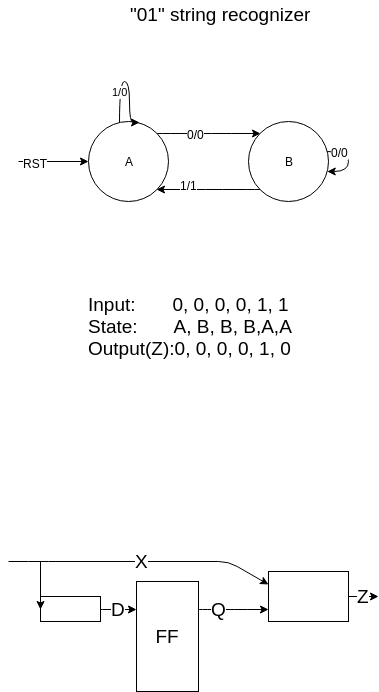
\includegraphics[width=0.6\textwidth]{state_machine}
	\caption{State Machine Example}
	\label{fig:state_machine}
\end{figure}

\subsection*{Lecture Notes}
\begin{itemize}
	\item Linux on Pynq: half Ubuntu, half Petalinux
	\item Should have most common packages
	\item Petalinux has BSP for Zynq
	\item Kernel has drivers for AXI busses etc. and writing to PL
	\item Overlay: a hardware library to be written to the PL
\end{itemize}

\subsection*{Overlays}
\begin{itemize}
	\item Programmable FPGA IP core
	\item IP bitstream
	\item C code to expose functionality
	\item Python wrapper for c code
	\item Base overlay: access to headers, buttons, switches, leds, PMODs, audio etc.
	\item Base overlay designed in Vivado (components reusable for other designs)
	\item Base overlay has Microblaze for each PMOD interface and one for Arduino header
	\item Overlay usually includes: bitstream, TCL script to determine IP, Python API
\end{itemize}


\end{document}
